\section{Remote Memory Access: MPI 3.0}
In the reign of parallel computing, there exist two major approaches for communicating data between processes:
message passing and direct memory access of the remote process. Shared memory approach is also there but that 
is limited to the procesess on the same node. 

MPI-1 provides a way for message passing between processes while MPI-2 gives approach for direct memory access of remote processes and MPI-3 extends it to a great extent. MPI RMA \cite{rmabook} uses operations like \textit{put}, \textit{get} and \textit{accumulate} to \textit{write}, \textit{read} and \textit{reduce} data respectively to a remote process without involving the remote process. One limitation of RMA approach is this it require special hardware support but with increasingly high development in networking caters this need to much extent.

\subsection{Shared memory vs RMA}
MPI remote memory access must be distinguished from shared memory programming model in the following ways:
\begin{itemize}
    \item MPI RMA approach can be used for communication between cores on the same node as well as cores on different
    nodes. While shared memory approach is limited to processes on the same core using \textit{threads}.
    \item In MPI RMA data can be accesses using {\ttfamily MPI\_Put} and {\ttfamily MPI\_Get} operations while in shared memory we can access data using usual load and store operations as shown in the pictures.
    \item In shared memory, we have a single address space, shared by multiple threads of execution while in RMA, programmer
    decides how much memory will be exposed to the remote process for communication. 
\end{itemize}
\begin{figure}
    \centering
    \begin{minipage}{.5\textwidth}
        \centering
        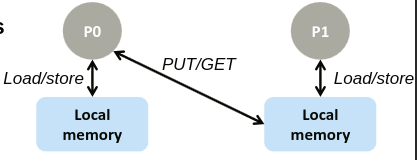
\includegraphics[width=0.78\linewidth]{attachments/rma.png}
        \caption{RMA$^1$}
    \end{minipage}%
    \begin{minipage}{.5\textwidth}
        \centering
        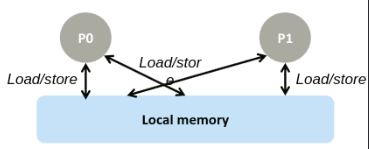
\includegraphics[width=0.78\linewidth]{attachments/shared_mem.png}
        \caption{Shared Memory$^1$}
    \end{minipage}
\end{figure}
The major disadvantage of shared memory model is \textit{simultaneous access by different threads to a same memory location.}
In order to avoid this race condition, many sophisticated techniques in compilers and special routines are needed such as 
\textit{locks and mutexes.}

\section{Introduction to RMA}
In traditional message passing, one process \textit{sends} data to other process using {\ttfamily MPI\_Send} and other 
process \textit{receives} data using {\ttfamily MPI\_Recv}. Every \textit{send} is compulsory to have a \textit{receive}
at the receiver process. This cooperative nature of MPI can impose order or need \textit{tag} matching for delivery of data
and that will have performance costs due to overheads.

MPI RMA provides a way of data communication from \textit{origin process} (process that sends data) to the \textit{target
process} (process to which data has been sent), without the involvement of \textit{target process}. The calling process specifies
both send and receive buffer. Since a single process is involved, these routines are also called \textit{one-sided routines}:

There are three main steps in using RMA:
\begin{itemize}
    \item \textbf{Defining a memory window:}\\
    Memory \textit{window} is collection of memory locations defined by a group of processes and only those locations can be
    modified by the remote process using RMA operations. This involves creation of a new MPI object {\ttfamily MPI\_Win}. There
    are $4$ window creation routines specified by MPI Forum.
    \item \textbf{Moving the data from \textit{origin} to \textit{target} process:}\\
    There are several routines to move the data between processes without the involve of the process instead directly writing the
    data into remote processes memory. These routines include: {\ttfamily MPI\_Put, MPI\_Get, MPI\_Accumulate} etc.
    \item \textbf{Specifying how do we know that data is available to remote process:}\\
    This is to say that how do we know that receive has been completed? There are several routines such as {\ttfamily MPI\_Win\_fence,
    MPI\_Win\_lock/unlock} etc. that makes sure that data is available to the target process for its local load/store operations.     
\end{itemize}

\subsection{Memory Window}
\begin{figure}[!ht]
    \centering
    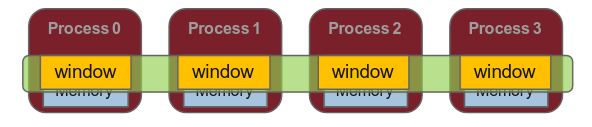
\includegraphics[width=0.75\linewidth]{attachments/mem_window.png}
    \caption{Memory window in RMA$^1$}
\end{figure}
It is the memory region of a process that can be accessed by another process using RMA operations. All or a group of processes can 
create a window or many windows by contributing some part of their memory to the window. It is a contiguous section of memory. There
are these $4$ window creation routines:
\begin{itemize}
    \item {\ttfamily MPI\_Win\_allocate:} In this routine memory allocation and window creation both are handled by MPI implemention.
    \item {\ttfamily MPI\_Win\_create:} This routine creates the window from already allocate memory. User have to provide some allocated
    memory to be create as a window.
    \item {\ttfamily MPI\_Win\_allocate\_shared:} This routine helps in creating a shared memory window from already allocate memory for
    the process on the same node hence these process can access each other data with simple load/store and avoid communication completely.
    \item {\ttfamily MPI\_Win\_create\_dynamic:} It creates a window but does not attach memory directly to it. Memory can be attached later
    using {\ttfamily MPI\_Win\_attach} and can be deattached using {\ttfamily MPI\_Win\_deattach}. 
\end{itemize}

By default, the memory that has been allocated by MPI implemention (if user specifies so) is {ttfamily contiguous} unless the
the {\ttfamily non-contiguous} option is {\ttfamily true.} This can have performance implications as well since {\ttfamily non-contiguous}
memory can be allocated aligning to the cache sizes which will decrease the number of cache misses.

After all the communication has been done and window is no longer required, it can be free using {\ttfamily MPI\_Win\_free} by all the 
processes that have created the window.\\
\hrule
\begin{listing}[!ht]
\begin{minted}[linenos]{Julia}
int MPI_Win_create(void *base, MPI_Aint size, int disp_unit,
                   MPI_nfo info, MPI_Comm comm, MPI_Win *win)
int MPI_Win_free(MPI_Win *win)
\end{minted}
\caption{Syntax for C}
\end{listing}
\hrule
\vspace{10pt}
There are few interesting parameters that are required by window calling routines:
\begin{itemize}
    \item \textbf{disp\_unit:} This argument unit should be the multiple of {\ttfamily sizeof()} of simple type such as `int` etc.
    that creates up the window object. For example if an array of {\ttfamily Floats} is making up the window then {\ttfamily disp\_unit}
    should be multiple of {\ttfamily sizeof(Float)}. This is the local unit size for displacements, in bytes.
    \item \textbf{info:} This arguemnt of only used for optimization purposes. A value {\ttfamily MPI\_INFO\_NULL} is always valid.
\end{itemize}

\subsection{Moving Data}
Since we have now seen how to make memory as a window for RMA opertaions, we need to specify how to move data between process.
MPI provides several routines to specify what data to move and to which location. Three of the simplest routines have been
described below:
\subsubsection{{\ttfamily \large MPI\_Put}}
\begin{figure}[!ht]
    \centering
    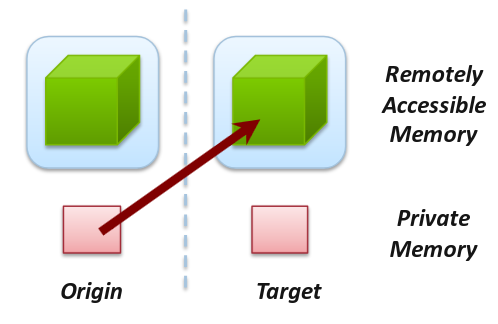
\includegraphics[width=0.35\linewidth]{attachments/put_rma.png}
    \caption{MPI\_Put$^1$}
\end{figure}
{\ttfamily MPI\_Put} is like a "store/write to remote memory" operation. It is a non-blocking communicating routine. This routines 
writes data from {\ttfamily origin} process's memory called {\ttfamily origin address} to {\ttfamily remote} process's memory at
the location as described by {\ttfamily displacement} argument. The data that need to be moved can be anywhere in the {\ttfamily origin}
process's memory, it need not to be inside a window.

Programmer need to pay attention while providing the {\ttfamily displacement} argument. \textbf{The destination of data is always relative
to the memory window exclusive to {\ttfamily remote} process not with the whole window object}.

MPI RMA operations define a separation between moving of data and completion of the operations. Window ~synchronization ~routines ~such as
{\ttfamily MPI\_Win\_fence} should be used after RMA opertions for completion of these operations. Between two {\ttfamily MPI\_Win\_fence} calls
any number of {\ttfamily MPI\_Put} operations can be issued. But if a {\ttfamily MPI\_Put} and {\ttfamily MPI\_Accumulate} operation overlaps (issued 
to same memory location) between two {\ttfamily MPI\_Win\_fence} calls then result will be {\ttfamily undefined behaviour.} Along with that,
{\ttfamily MPI\_Put} and {\ttfamily MPI\_Get} both can not be used within two {\ttfamily MPI\_Win\_fence} calls.

{\ttfamily MPI\_Put} is \textbf{not} an atomic operation. An \textbf{atomic operation} is an operation that can be completed within one CPU cycle and
hence these operation can not be interrupted in between by any other process. They execute at lowest level and cannot be broken further.
\begin{listing}[!ht]
\hrule \vspace{5pt}
\begin{minted}[linenos]{Julia}
int MPI_Put(const void *origin_addr,
            int origin_count, MPI_Datatype origin_datatype, int
            target_rank, MPI_Aint target_disp, int target_count,
            MPI_Datatype target_datatype, MPI_Win win)
\end{minted}
\caption{Syntax for C}
\hrule
\end{listing}

\subsubsection{{\ttfamily \large MPI\_Get}}
\begin{figure}[!ht]
    \centering
    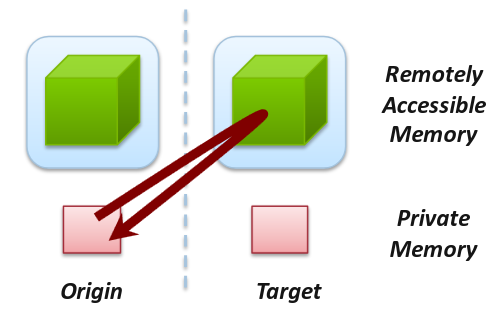
\includegraphics[width=0.35\linewidth]{attachments/get_rma.png}
    \caption{MPI\_Get$^1$}
\end{figure}
{\ttfamily MPI\_Get} routine is used to get data from remote process to the calling process. It can get data from remote process's window to anywhere 
in the origin (calling) process memory means {\ttfamily origin\_addr} need not to be inside window for calling process. This operation is also not an
\textbf{atomic} operation.\\
While calling this routine, programmer needs to specify the {\ttfamily displacement} argument relative to the window exclusive to the remote process.

This displacement arguement will specify the location of the data at remote process that needs to be written at the origin process's memory. After
using this routine, there should be a call to a window synchronization routine to ensure that the data has been received at the origin process.
\begin{listing}[!ht]
\hrule \vspace{5pt}
\begin{minted}[linenos]{Julia}
int MPI_Get(void *origin_addr, int origin_count, 
            MPI_Datatype origin_datatype, int target_rank,
            MPI_Aint target_disp, int target_count,
            MPI_Datatype target_datatype, MPI_Win win)
\end{minted}
\hrule
\caption{Syntax for C}
\end{listing}

\subsubsection{{\ttfamily \large MPI\_Accumulate}}
\begin{figure}[!ht]
    \centering
    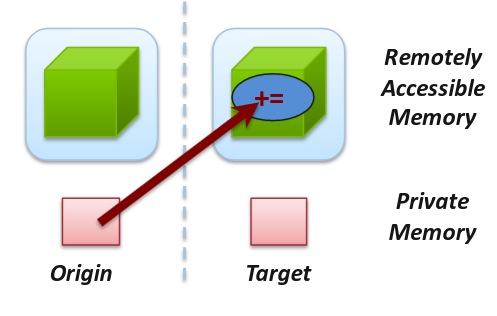
\includegraphics[width=0.35\linewidth]{attachments/accum_rma.png}
    \caption{MPI\_Accumulate$^1$}
\end{figure}
{\ttfamily MPI\_Accumulate} routine provides a way to move and combine data at the target process using any of the reduction operations such as
{\ttfamily MPI\_SUM, MPI\_MAX} etc. It can be seen similar to {\ttfamily MPI\_Reduce} operation but without the involvement of target process. There
are few restrictions for using {\ttfamily MPI\_Accumulate} as listed below:
\begin{itemize}
    \item It allows \textbf{only predefined operations} such as {\ttfamily MPI\_SUM, MPI\_MAX, MPI\_MIN, MPI\_LAND, MPI\_LOR} etc.
    \item It allows only \textbf{predefined} MPI datatypes and MPI derived datatypes where all components are of same predefined datatype.
\end{itemize}
\subsubsection{{\ttfamily MPI\_Accumulate as MPI\_Put}}
Since {\ttfamily MPI\_Accumulate} is an atomic operation while {\ttfamily MPI\_Put} is not an atomic operation and if we want to use atomic
{\ttfamily  MPI\_Put} we can achieve this using {\ttfamily MPI\_Replace} as an operation of {\ttfamily MPI\_Accumulate}. This will put the value in {\ttfamily origin\_addr} buffer to the target location as provided while calling this routine.

\begin{listing}[!ht]
\hrule \vspace{5pt}
    \begin{minted}[linenos]{Julia}
int MPI_Accumulate(const void *origin_addr, int origin_count,
                MPI_Datatype origin_datatype, int target_rank,
                MPI_Aint target_disp, int target_count,
                MPI_Datatype target_datatype, MPI_Op op,
                MPI_Win win)
    \end{minted}
\hrule
    \caption{Syntax for C}
\end{listing}

\subsection{Synchronization Routines}
Synchronization routines are a way to tell the process that data is available for local load/store operations from RMA operations as well as data is available for RMA operations from local load/store operations. They need to be called before as well as after RMA operations. The reason for calling them before RMA operations is to make sure that any local load/store operation that had been performed on the window object has been successfully completed and that data can be used in RMA operations. This can be omitted if there are no local load/store operations on the window before RMA operations. Later calling them will make sure the completion of RMA opertions itself.

There are two types of target synchronization in MPI RMA:
\begin{enumerate}
    \item Active Target synchronization.
    \item Passive Target synchronization.
\end{enumerate}

\subsubsection{\large Active Target synchronization} 
Active target synchronization involves both the origin and the target processes in synchronization using {\ttfamily MPI\_Win\_fence}. Any MPI RMA calls need to be wrapped by {\ttfamily MPI\_Win\_fence} call.

\subsubsection{\textbf{MPI\_Win\_fence}}
{\ttfamily MPI\_Win\_fence} is a collective call to all processes in the group associated with the window object that has been passed to {\ttfamily MPI\_Win\_fence}. It makes sure that any local stores to the memory window will be visible to RMA operations before any RMA operation takes place. In any pair of successive {\ttfamily MPI\_Win\_fence} there may either be any local stores to the local memory window or {\ttfamily  MPI\_Put/Accumulate} calls but not both.If there no {\ttfamily MPI\_Put} operation in between two {\ttfamily MPI\_Win\_fence} call then there may be both load and {\ttfamily MPI\_Get} operations on the memory window. 

{\ttfamily assert} argument can be used to indicate exactly what kind of operation \linebreak{\ttfamily MPI\_Win\_fence} is synchronizing. Typically, it is used to separate {\ttfamily MPI\_Put/Accumulate} operations from local load and store operation. \vspace{10pt}
\hrule \vspace{-8pt}
\begin{minted}[linenos]{Julia}
int MPI_Win_fence(int assert, MPI_Win win)        
\end{minted}
\vspace{-8pt}
\hrule

\subsubsection{\large Passive Target synchronization}
In this synchronization, the target process does not need to call any synchronization routines such as {\ttfamily MPI\_Win\_fence}. Before starting any RMA call, there should be a {\ttfamily MPI\_Win\_lock} and after those calls there should be a {\ttfamily MPI\_Win\_unlock} but only on the origin proce. This means that all the RMA calls will get completed after {\ttfamily MPI\_Win\_unlock} returns.

{\ttfamily MPI\_Win\_unlock} ensures that the RMA operations have been completed successfully and all the data transfers are visible to the target memory esssentially all the synchronization is done by {\ttfamily MPI\_Win\_unlock}. There is another version of lock that locks the window on all the processes called {\ttfamily MPI\_Win\_lock\_all}. {\ttfamily MPI\_Win\_unlock\_all} is used to unlock the window then. But there is some restrictions on type of lock used for {\ttfamily MPI\_Win\_lock\_all}, it can only provide shared access using {\ttfamily MPI\_LOCK\_SHARED} and the exclusive.

{\ttfamily MPI\_Win\_lock} call is in itself a {\em non-blocking} call hence it will return the control to the calling process just after the call and it will not wait for the target process to {\em acquire} the lock except in the case when the target process is same as the calling process, there MPI standard specifies it to be a {\em blocking} call. 

Since {\ttfamily MPI\_Win\_unlock} performs the synchronization and that will be called at the end. But what if we want to use the communicated data before calling {\ttfamily  MPI\_Win\_unlock}? In that case, there are few routines available for synchronization before calling {\ttfamily MPI\_Win\_unlock}.\\
For Separate Memory Model: \footnote[2]{For memory models, see section \ref{model}}
\begin{itemize}
	\item {\ttfamily MPI\_Win\_flush}: This routine can do force completion of all RMA routines that has been called till that point, both at the `origin` as well as on target process.
	\item {\ttfamily MPI\_Win\_flush\_local}: This routine can complete all RMA operations locally for the process which is calling the RMA operations.
\end{itemize}
Hence, the buffers involved in pending RMA operations at the origin process can be re-used safely after calling above routine.\\
For Unified Memory Model: \footnotemark[2]
\begin{itemize}
	\item {\ttfamily MPI\_Win\_sync}: It synchronizes private memory with public memory window in passive RMA.
\end{itemize}
Unified model is indeed coherent but the timings of when the updates of public memory become visible in private memory is not explicitly defined hence it is advisable to use this function. \vspace{10pt}
\hrule \vspace{5pt} \hspace{-21pt}
\textbf{Note:}\\
Writing RMA program by having a memory model in mind may limits portability hence prefer {\ttfamily MPI\_Win\_flush} operation as they are available on both models. \vspace{5pt}
\hrule

\subsection{Memory models} \label{model}
\textbf{Separate memory model}\\
The entire RMA implementation is based on the concept of public and private memory. Local load and store operations use private memory while the RMA operations uses public (exposed) memory. In separate memory model, the private and public memory remains logically separated and public memory window holds copy of the variable from private memory. These type of model is generally used on \textbf{non-coherent} systems.

{\ttfamily MPI\_Win\_fence} essentially makes the sure that whatever changes were made to public memory has been copied to private memory as vice-versa. Different values of assert parameter can be provided to avoid unnecessary copying.The above reasoning also says that only RMA routines must be used to update memory location in window object.
\begin{figure}[!ht]
    \centering
    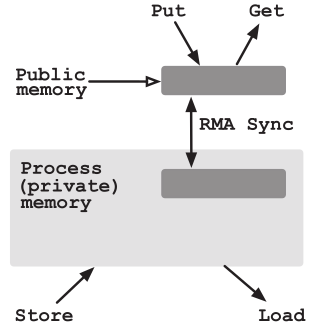
\includegraphics[width=0.35\linewidth]{attachments/sep_mem_model.png}
    \caption{Separate Memory Model$^1$}
\end{figure}\\
\vspace{3pt} \hspace{-11pt}
\textbf{Unified memory model}\\
In coherent systems, MPI implementations does not differentiate between the public and private memory i.e. changes made to private memory location will eventually become visible to public memory but the keyword here is {\em eventually}.

Hence programmers are advised to make sure the visibility of changes by using synchronization routines such as {\ttfamily MPI\_Win\_fence}, {\ttfamily MPI\_Win\_unlock} or {\ttfamily MPI\_Win\_Sync}
\begin{figure}[!ht]
    \centering
    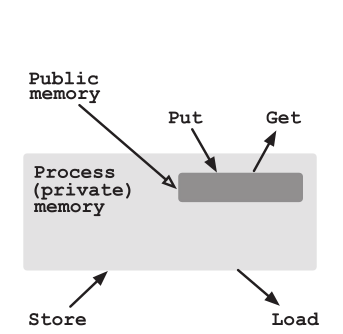
\includegraphics[width=0.37\linewidth]{attachments/uni_mem_model.png}
    \caption{Unified Memory Model$^1$}
\end{figure}
\hrule \vspace{5pt} \hspace{-21pt}
\textbf{Note:}\footnotetext[1]{All images credits: \cite{rma}}\\
To determine whether the MPI environment provides the unified or separate memory model, one can check the the MPI\_WIN\_MODEL attribute on the window. The value of this attribute is a pointer to an integer that can have one of two values: MPI\_WIN\_UNIFIED or MPI\_WIN\_SEPARATE for the unified and separate memory models, respectively.

\section{Implementation} \label{i}
In this section, we will discuss about the implementation of classical Lax-Wendroff method for linear advection equation using finite difference approach in 1D case. The theory related to finite difference approach can be found in section \ref{fdm} of chapter \ref{tf}. This is the parallel code implemented using MPI RMA.
\begin{minted}[linenos]{Julia}
# getting boundary values and halo exchanges
function get_ghost_values!(param, u, win)
    if size == 1
        u[1] = u[param.N_local]
        u[param.N_local + 2] = u[3]
        return
    end
    next = (rank + 1) % size
    if rank !== size - 1  
        buf1 = fill(0.0, 1)
        MPI.Win_lock(win; rank=next, type=MPI.LOCK_SHARED, nocheck=true)
        MPI.Put!(u[param.N_local+1], win; rank=next, disp=0)
        MPI.Get!(buf1, win; rank=next, disp=1)
        MPI.Win_unlock(win, rank=next)
        u[N_local+2] = buf1[1]
    else
        buf2 = fill(0.0, 1)
        MPI.Win_lock(win; rank=next, type=MPI.LOCK_SHARED, nocheck=true)
        MPI.Put!(u[param.N_local], win; rank=next, disp=0)
        MPI.Get!(buf2, win; rank=next, disp=2)
        MPI.Win_unlock(win; rank=next)
        u[N_local+2] = buf2[1]
    end
    MPI.Win_fence(win)
end
\end{minted}
The above code is writtten for periodic boundary conditions. {\ttfamily get\_ghost\_values!} function is the only function that required MPI communication and rest all code is serial. In above function, the first {\ttfamily if} block is to handle the case if total number of processes is 1 essentially the serial case. Now, talking about the main part related to MPI RMA, we are using {\ttfamily lock/unlock} mechanism hence this is passive target synchronization.

{\ttfamily MPI\_Put} has been used to write the values from {\ttfamily u[param.N\_local+1]} to the {\ttfamily next} rank at the displacement 0 means at the starting of the window of {\ttfamily next} rank. Then {\ttfamily MPI\_Get} has been used to get the values from {\ttfamily next} rank's displacement 1 to the buffer {\ttfamily buf1}. The displacement 1 simply means that we need to skip the first memory location in the window of the {\ttfamily next} rank. 

At the end, {\ttfamily MPI\_Win\_fence} is used in order to complete the store operations that we are performing at the location {\ttfamily u[N\_local+2]}. We can also omit the use of {\ttfamily MPI\_Get} completely and can just use {\ttfamily MPI\_Put}. By doing this, we also not need to perform the store operation at the last hence no need to use {\ttfamily MPI\_Win\_fence}. {\ttfamily nocheck=true} is an optimization option that will skip the check for access to the window by other processes as we know that the code is written in such a way that there won't be any illegal access attempts to the window. The optimization in MPI RMA is the responsibility of the programmer by providing such options. This is not the most optimized code and it can further be optimized. 

The reader should not get confused with {\ttfamily if} conditions as they are required due to periodic boundary conditions and subject to change as depends on boundary condition used.

In this project, I have also implemented the serial and parallel (MPI RMA) implementation of linear advection equation in 1D and 2D cases and is available on Github on this \href{https://github.com/Devansh1106/Sample-MPI-Julia/tree/main/linadv}{link.} 
\begin{center}
    \rule{3cm}{1pt}
\end{center}